%
% grundlagen.tex -- Grundlagen ueber Differentialgleichungen
%
% (c) 2015 Prof Dr Andreas Mueller, Hochschule Rapperswil
%
\chapter{Grundlagen der Theorie der gew"ohnlichen Differentialgleichungen
\label{chapter:grundlagen}}
\rhead{}
\lhead{Grundlagen}
\section{Differentialgleichungen\label{section:differentialgleichungen}}
\rhead{Differentialgleichungen}
Eine gew"ohnliche Differentialgleichung f"ur eine reellwertige
Funktion $y(x)$ stellt einen Zusammenhang her zwischen der Funktion
und ihren Ableitungen.
Wir schreiben die Ableitungen als $y'$, $y''$, $y'''$ und $y^{(n)}$
f"ur die $n$-te Ableitung.
Wir lassen oft das Argument der Funktion weg.
Beispiele von Differentialgleichungen sind
\begin{align*}
y'&=-Ny
&&\text{Ordnung: $1$}
\\
y''&=-\omega^2 y
&&\text{Ordnung: $2$}
\\
x^2y''+xy'+(x^2-n^2)y&=0
&&\text{Ordnung: $2$}
\end{align*}
Die Abh"angigkeit kann in expliziter Form als
\begin{equation}
y^{(n)}=f(x,y,y',\dots,y^{(n-1)})
\label{grundlagen:explizit}
\end{equation}
oder in impliziter Form
\[
F(x,y,y',\dots,y^{(n)})=0
\]
gegeben sein.
Die Ordnung einer Differentialgleichung ist die h"ochste vorkommende
Ableitung.

\begin{figure}
\centering
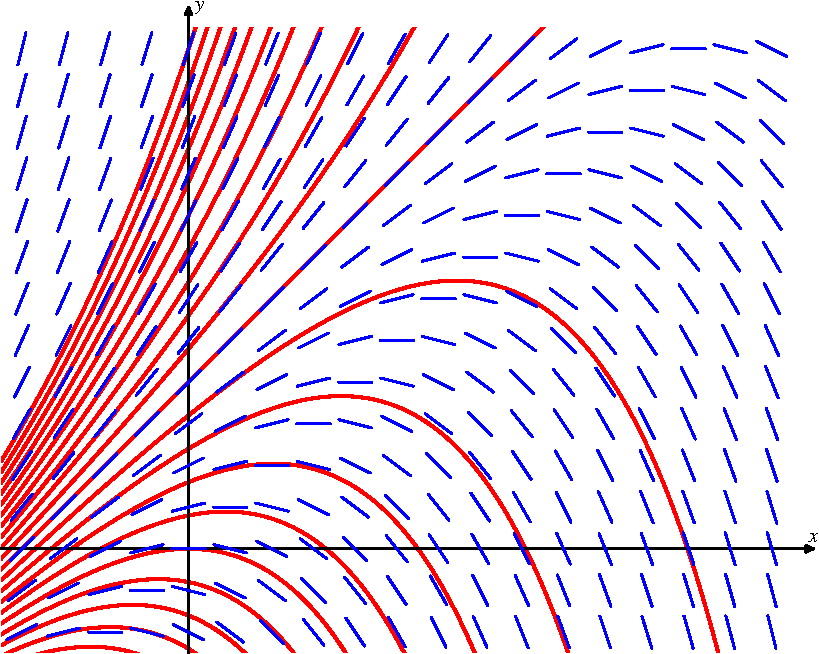
\includegraphics{chapters/images/grundlagen-1.pdf}
\caption{Richtungsfeld der Differentialgleichung $y'=y-x$ mit
einzelnen L"osungskurven.
\label{grundlagen:richtungsfeld}}
\end{figure}%

Differentialgleichungen erster Ordnung lassen sich mit Hilfe eines
Richtungsfeldes visualisieren, wie in Abbildung~\ref{grundlagen:richtungsfeld}
dargestellt.
In jedem Punkt $(x,y)$ der $x$-$y$-Ebene wird die Steigung $y'=f(x,y)$
eingezeichnet.
Eine L"osung der Differentialgleichung hat in diesem Bild als Graph
eine Kurve in der $x$-$y$-Ebene, die an jeder Stelle als Tangente 
das Richtungsfeld haben.

Insbesondere in Anwendungen in der Physik ist die Zeit die
unabh"angige Variable.
Die abh"angige Variable ist dann zum Beispiel die Ortskoordinate
$x(t)$ und wir bezeichnen ihre Ableitungen mit $\dot{x}(t)$ f"ur
die Geschwindigkeit, $\ddot{x}(t)$ f"ur die Beschleunigung.
Dieses Beispiel suggeriert auch, dass die abh"angige Variable 
ein Vektor sein kann, den man als den Ortsvektor eines Teilchens
interpretieren kann.
Auch die Funktion $f(t,x,\dots,x^{(n-1)})$ muss dann vektorwertig sein, und
ebenso alle Argumente ausser dem ersten von $f$.

Eine Differentialgleichung $n$-ter Ordnung f"ur eine skalare Funktion
kann in eine Vektor-Differen\-tialgleichung erster Ordnung f"ur eine
$n$-dimensionale vektorwertige Funktion umgewandelt werden.
Ist $y(x)$ die gesuchte Funktion in der
Differentialgleichung~(\ref{grundlagen:explizit}), dann kann man
den Vektor
\[
u(x)=\begin{pmatrix}
y(x)\\y'(x)\\\vdots\\y^{(n-1)}(x)
\end{pmatrix}
\in\mathbb R^n
\]
bilden.
Er erf"ullt die Differentialgleichung
\begin{equation}
\frac{d}{dx}\begin{pmatrix}
y\\y'\\\vdots\\y^{(n-1)}
\end{pmatrix}
=
\begin{pmatrix}
y'\\y''\\\vdots\\y^{(n)}
\end{pmatrix}
=
\begin{pmatrix}
y'\\y''\\\vdots\\f(x,y,y',\dots,y^{(n-1)})
\end{pmatrix}.
\label{grundlagen:vektordgl}
\end{equation}
Der Vektor auf der rechten Seite h"angt nur von $x$, der Funktion $y$
und ihren Ableitungen bis zur $n-1$-ten Ordnung ab, also von $u$, man
kann (\ref{grundlagen:vektordgl}) daher als
\begin{equation}
\frac{d}{dx}u=\tilde{f}(x,u)
\end{equation}
schreiben.
Im Folgenden werden wir fast ausschliesslich Differentialgleichungen
erster Ordnung der Form $y'=f(x,y)$ betrachten, und dabei stillschweigend
zulassen, dass $y$ ein Vektor ist.

Differentialgleichungen h"oherer Ordnung oder Vektordifferentialgleichungen
lassen sich nicht so einfach visualisieren wie Differentialgleichungen
erster Ordnung.
Ist $y(x)$ eine L"osung der Vektor-Differentialgleichung $y'=f(x,y)$
mit $y\in\mathbb R^n$, dann ist die Abbildung
\[
\gamma\colon
x\mapsto\begin{pmatrix}
x\\
y(x)
\end{pmatrix}\in\mathbb R^{n+1}
\]
eine Kurve im $n+1$-dimensionalen Raum. 
Der Tangentialvektor ist
\begin{equation}
\gamma'(x)
=
\begin{pmatrix}1\\y'(x)\end{pmatrix}
=
\begin{pmatrix}1\\f(x,y(x))\end{pmatrix}.
\label{grundlagen:gamma-vektorfeld}
\end{equation}
Die Kurve $\gamma(x)$ ist also in jedem Punkt des $n+1$-dimensionalen
Raumes tangential an das Vektorfeld, welches
durch~(\ref{grundlagen:gamma-vektorfeld}) definiert wird.
Der Spezialfall $n=1$ f"uhrt wieder zur"uck auf das Richtungsfeld
wie in Abbildung~\ref{grundlagen:richtungsfeld}.

\subsection{Anfangswertprobleme\label{section:anfangswertprobleme}}
Die Differentialgleichung $y'=f(x,y)$ alleine kann eine L"osungsfunktion
$y(x)$ nicht festlegen, sie codiert nur, wie sich die L"osung ver"andern wird.
Es ist also zus"atzlich die Angabe eines Punktes der L"osungskurve
notwendig.
Man nennt das Problem, eine Funktion $y(x)$ zu finden, welche
\[
y'=f(x,y)
\qquad
\text{und}
\qquad
y(0)=y_0
\]
erf"ullt, ein {\em Anfangswertproblem}.
Ein Anfangswertproblem verlangt f"ur die gew"ohnliche Differentialgleichung
$n$-ter Ordnung verlangt also die Angabe der Werte von
$y(0),y'(0),\dots,y^{(n-1)}(o)$

\subsubsection{Existenz und Eindeutigkeit von L"osungen}
Die Existenz und Eindeutigkeit einer L"osung ist aus den Beispielen und
graphischen Darstellungen intuitiv verst"andlich, f"ur einen exakten
Beweis sind jedoch zus"atzliche Voraussetzungen n"otig.

\begin{definition}
Eine Funktion $f\colon \mathbb R^n\to\mathbb R^m$ heisst global
{\em Lipschitz-stetig},
\index{Lipschitz-stetig}
wenn es eine Zahl $L$ gibt 
\begin{equation}
|f(x_2)-f(x_1)| \le L\,|x_2-x_1|
\label{grundlagen:lipschitz}
\end{equation}
f"ur alle Vektoren $x_1,x_2\in\mathbb R^n$.
Eine Funktion heisst lokal Lipschitz-stetig im Punkt $x_0$, wenn die
Bedingung (\ref{grundlagen:lipschitz}) f"ur $x_i$ in einer Umgebung von
$x_0$ erf"ullt ist.
\end{definition}

Eine Funktion ist insbesondere dann lokal Lipschitz-stetig, wenn sie
stetig differenzierbar ist.
In diesem Fall ist die Ableitung $f'(x)$ in einer Umgebung von $x_0$
beschr"ankt, also $|f(x)|<M$, und der Mittelwertsatz der Differentialgleichung
sagt, dass
\[
|f(x_2)-f(x_1)|\le M |x_2-x_2|
\]
ist, $f$ ist also lokal Lipschitz-stetig.

\begin{satz}[Picard-Lindel"of]
\label{grundlagen:picard-lindeloef}
Ist die Funktion $f(x,y)$ lokal Lipschitz-stetig bez"uglich der Variablen
$y$ f"ur $x\in[x_0,b]$ und $|y-y_0|<R$.
Dann hat das Anfangswertproblem
\[
y'(x)=f(x,y)\qquad\text{und}\qquad y(x_0)=y_0
\]
ein eindeutige L"osung, die in einem Intervall $[x_0,x_0+\varepsilon)$
definiert ist.
\end{satz}

In diesem Buch werden die Funktionen $f$ der Differentialgleichungen 
meistens stetig differenzierbar sein, so dass der
Satz~\ref{grundlagen:picard-lindeloef} in unseren Anwendungen die lokale
Existenz und Eindeutigkeit einer L"osung garantiert.

\subsection{Autonome Differentialgleichungen}
Eine besondere Bedeutung haben Differentialgleichungen, in denen
$f$ nicht von $x$ abh"angt, man nennt sie {\em autonom}
\index{autonome Differentialgleichung}.
Die L"osungen einer solchen Differentialgleichungen h"angen im
folgenden Sinne nicht vom Start-$x$-Wert ab:
Ist $y(x)$ die L"osung des Anfangswertproblems
\[
y'=f(y)\qquad\text{und}\qquad y(0)=y_0,
\]
dann ist die Funktion
\[
y_1(x)=y(x-x_0)
\]
L"osung des Anfangswertproblems
\[
y'=f(y)\qquad\text{und}\qquad y(x_0)=y_0.
\]
Etwas salopp kann man das auch so formulieren: f"ur den Verlauf der 
L"osungskurve kommt es nicht darauf an, wann die L"osungskurve bei 
einem Punkt vorbeikommt.
Der weitere Verlauf der L"osungskurve wird immer der gleiche sein,
unabh"angig davon, wann ein bestimmter Punkt besucht wird.

Die Darstellungen der L"osungskurven ohne die Angabe des
zugeh"origen $x$ sind daher f"ur autonome Differentialgleichungen
 aussagekr"aftig.
Wir nehmen im folgenden an, dass $f$ die Bedingungen f"ur Existenz
und Eindeutigkeit von L"osungen sowie f"ur die stetige Abh"angigkeit
von den Anfangsbedingungen erf"ullt.

\begin{figure}
\centering
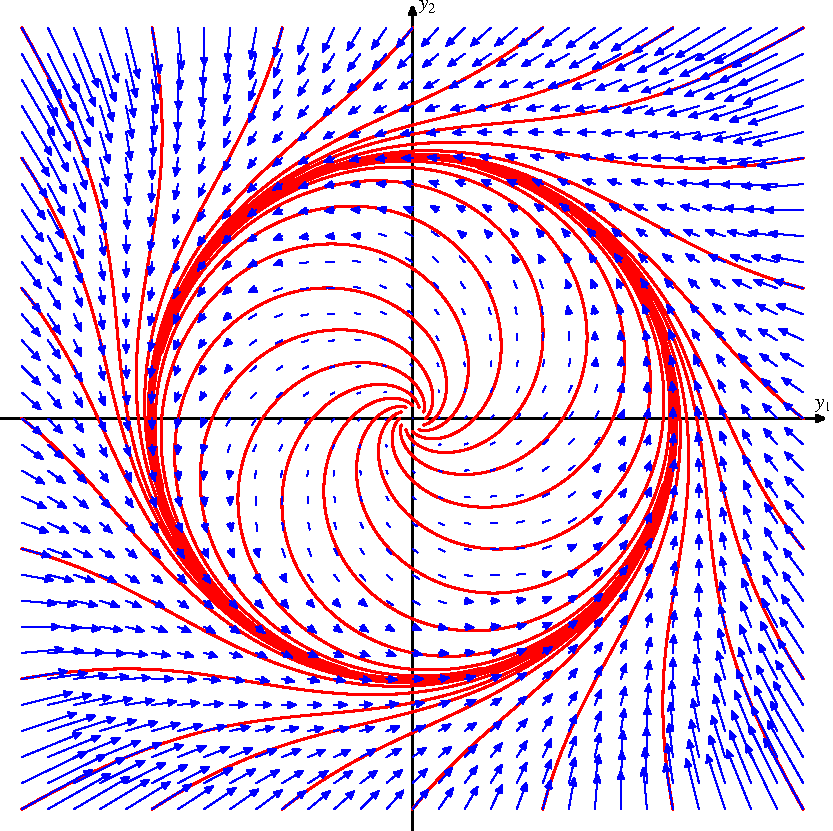
\includegraphics{chapters/images/grundlagen-2.pdf}
\caption{Vektorfeld des autonomen Differentialgleichungssystems
(\ref{grundlagen:hopfsystem})
mit L"osungskurven.
\label{grundlagen:vektorfeld}}
\end{figure}%

Eine autonome Differentialgleichung definiert in jedem Punkt des
Raumes, aus dem die $y$-Vektoren stammen, einen Vektor $f(y)$,
man spricht von einem {\em Vektorfeld}.
\index{Vektorfeld}
Indem wir in jedem Punkt des $y$-Raumes den Vektor $f(y)$ aufzeichnen,
k"onnen wir eine graphische Darstellung des Vektorfeldes erhalten
(Abbildung~\ref{grundlagen:vektorfeld}).
Die Bahn des Punktes $y(x)$ in Abh"angigkeit von $x$ ist eine Kurve,
deren Tangentialvektor in jedem Punkt der $y$-Ebene durch die Funktion
$f(y)$ gegeben ist.
In Abbildung~\ref{grundlagen:vektorfeld} ist das Vektorfeld des
Differentialgleichungssystems
\begin{equation}
\begin{aligned}
y_1'&=y_1-y_2-y_1(y_1^2+y_2^2)\\
y_2'&=y_1+y_2-y_2(y_1^2+y_2^2)
\end{aligned}
\label{grundlagen:hopfsystem}
\end{equation}
dargestellt.
Das Vektorfeld ist durch die Funktion $f(y)$ mit
\[
y=\begin{pmatrix}y_1\\y_2\end{pmatrix}
\qquad\text{und}\qquad
f(y)=\begin{pmatrix}
y_1-y_2-y_1(y_1^2+y_2^2)\\
y_1+y_2-y_2(y_1^2+y_2^2)
\end{pmatrix}
\]
gegeben.

Sehr viele Differentialgleichungen der Physik sind autonom.
Die unabh"angige Variable ist hier typischerweise die Zeit $t$, die
Naturgesetze, die Anlass zu den Differentialgleichungen geben,
h"angen nicht explizit von der Zeit ab. 
Zum Beispiel f"uhrt das Kraftgesetz der Gravitation auf die
Differentialgleichung
\[
m\ddot x=-\frac{GMm}{|x|^2}\frac{x}{|x|}
\]
f"ur die Bewegung eines Planeten der Masse $m$ um die Sonne mit Masse $M$.
Da die Massen konstant bleiben, tritt die Zeit auf der rechten Seite nicht
explizit auf.
Dies bedeutet auch, dass die Bahn immer gleich aussieht, unabh"angig
davon, wann der Planet startet.
In der Physik spricht man auch davon, dass die Bahn von einem 
Vektorfeld von Kraftvektoren $\vec F$ bestimmt wird.

F"ur eine autonome Differentialgleichung l"asst sich also zu jedem
Anfangspunkt eine L"osung finden.
Sind ausserdem die Voraussetzungen f"ur Existenz, Eindeutigkeit
und stetige Abh"angigkeit der L"osung von den Anfangsbedingungen erf"ullt,
k"onnen wir alle L"osungen in eine Funktion $\varphi$ zusammenfassen.
Sie ist definiert dadurch, dass
die Abbildung
\[
x\mapsto \varphi_x(y_0)
\]
L"osung des Anfangswertproblems
\[
y'=f(y)
\qquad\text{und}\qquad 
y(0)=y_0
\]
Wegen der Autonomie ist dann auch $y_{x-x_0}(y_0)$ L"osung des
Anfangswertproblems
\[
y'=f(y)
\qquad\text{und}\qquad 
y(x_0)=y_0,
\]
die Funktion $\varphi$ fasst also alle L"osungen in einer einzigen
Funktion zusammen.
Sie erf"ullt die Zusammensetzungsbedingung
\[
\varphi_{x_1+x_2}(y_0)=\varphi_{x_1}(\varphi_{x_2}(y_0)).
\]
Die Abbildung $\varphi$ heisst der {\em Fluss} des durch die autonome 
Differentialgleichung gegebenen Vektorfeldes.
\index{Fluss eines Vektorfeldes}

\subsubsection{Umwandlung in eine autonomes Problem}
Jede gew"ohnliche Differentialgleichung der Form
\begin{equation}
y'=f(x,y), \qquad y(0)=y_0
\label{skript:deautonom-dgl}
\end{equation}
kann in ein gleichbedeutendes autonomes Differentialgleichungssystem
umgewandelt werden.

Wir f"uhren zu diesem Zweck eine neue unabh"angige Variable $t$ ein,
und betrachten sowohl $x$ als auch $y$ als Funktionen von $t$. 
Die Funktion $f(x,y)$ h"angt nat"urlich nicht explizit von $t$ ab.
Die neue unabh"angige Variable soll sich nicht von $x$ unterscheiden,
wir fordern daher, dass $x$ die Differentialgleichung
\begin{equation}
\frac{dx}{dt}=1,\qquad x(0)=0
\label{skript:deautonom-param}
\end{equation}
erf"ullt ist, die wir sofort l"osen k"onnen: $x(t)=t$.
Wenn wir zur Differentialgleichung (\ref{skript:deautonom-dgl}) 
die Differentialgleichung (\ref{skript:deautonom-param}) hinzunehmen,
bekommen wir ein Differentialgleichungssystem, dessen rechte Seite
nicht explizit von  $t$ abh"angt.

Wir fassen $x$ und $y$ in einen $n+1$-dimensionalen Vektor $Y$ zusammen,
also
\[
Y
=
\begin{pmatrix}x\\y\end{pmatrix}
=
\begin{pmatrix}x\\y_1\\\vdots\\y_n\end{pmatrix}.
\]
Ausserdem schreiben wir
\[
F(Y)
=
\begin{pmatrix}1\\f(x,y)\end{pmatrix}
=
\begin{pmatrix}1\\f_1(x,y)\\\vdots\\f_n(x,y)\end{pmatrix},
\qquad
Y_0
=
\begin{pmatrix}0\\y_0\end{pmatrix}
=
\begin{pmatrix}0\\y_{0,1}\\\vdots\\y_{0,n}\end{pmatrix}.
\]
Mit dieser Notation ist das Differentialgleichungssystem
\[
\frac{d}{dt}Y=F(Y),\qquad Y(0)=Y_0
\]
ein autonomes System, welches die gleiche L"osung hat wie das
urspr"ungliche System.

\begin{satz}
Das $n$-dimensionale Differentialgleichungssystem 
\[
\frac{dy}{dx}=f(x,y)
\]
ist dem $n+1$-dimensionalen {\em autonomen} Differentialgleichungsssystem
\[
\frac{d}{dt}
\begin{pmatrix}
x\\y
\end{pmatrix}
=
\begin{pmatrix}1\\f(x,y)\end{pmatrix}
\]
"aquivalent.
\end{satz}

Die Tatsache, dass die Dimension des Systems erh"oht wird, hat tiefgreifende
Konsequenzen f"ur die m"oglichen L"osungen.
Zum Beispiel zeigt der Satz von Poincar\'e-Bendixson dass ein zweidimensionales
autonomes System keine chaotischen Bahnen haben kann.
Ein beliebiges eindimensionales System ist "aquivalent zu einem
zweidimensionalen autonomen System, also kann man in einem eindimensionalen
System kein chaotisches Verhalten beobachten.
Chaos verlangt nach einem autonomen System, welches mindestens dreidimensional
ist.
Oder einem beliebigen System mindestens von Dimension 2.

\subsection{Randwertprobleme\label{section:randwertprobleme}}
Wenn man einen Ball wirft, wird seine Bewegung durch die
Vektordifferentialgleichung zweiter Ordnung
\[
\frac{d^2}{dt^2}\begin{pmatrix}x\\y\end{pmatrix}
=
\begin{pmatrix}0\\\displaystyle-\frac{g}{m}\end{pmatrix}
\]
beschrieben.
Die Bahn ist ausserdem bestimmt durch die Anfangsbedingungen,
d.~h.~also den Anfangspunkt und die Anfangsgeschwindigkeit der Bahn.
Praktischer Ballwurf verlangt aber, dass ein Ziel erreicht wird.
Die Aufgabenstellung ist daher eine Bahnkurve $\gamma(t)$ zu finden,
welche sowohl durch den Anfangspunkt als auch den Zielpunkt
verl"auft.

Die L"osung einer Differentialgleichungen erster Ordnung f"ur eine
unbekannte reellwertige Funktion $y(x)$ ist vollst"andig durch einen
einzigen Anfangswert bestimmt.
Eine Differentialgleichung zweiter Ordnung f"ur eine unbekannte
rellwertige Funktion $y(x)$ verlangt dagegen zwei Anfangswerte,
n"amlich f"ur $y(0)$ und $y'(0)$.
In Analogie zum Problem des Ballwurfs k"onnte die L"osungsfunktion auch
festgelegt werden durch den Wert f"ur $x=0$ und $x=1$.
Gesucht ist also eine Funktion $y(x)$ auf dem Intervall $[0,1]$, die
\begin{equation}
y''=f(x,y,y')
\qquad\text{mit}\qquad
y(0)=y_0,
\qquad
y(1)=y_1
\end{equation}
erf"ullt.

\begin{beispiel}
Wir l"osen die Differentialgleichung $y''=-y$ mit den Randwerten
$y(0)=1$ und $y(1)=2$.
Die homogene Differentialgleichung hat die Funktionen
\[
y(x)=A \cos x + B\sin x
\]
als allgemeine L"osung.
Die Konstanten $A$ und $B$ m"ussen so gew"ahlt werden, dass die Randwerte
korrekt sind.
Setzt man $x=0$ und $x=1$ ein, erh"alt man die linearen Gleichungen
\begin{align*}
a=y(0)&=A\cos 0 + B\sin 0=A\\
b=y(1)&=A\cos 1 + B\sin 1
\qquad\Rightarrow\qquad
\frac{b-a\cos 1}{\sin 1}.
\end{align*}
Die L"osung des Randwertproblems ist daher die Funktion
\[
y(x)=a\cos x +\frac{b-a\cos 1}{\sin 1}\sin x,
\]
wie man auch durch Einsetzen von $x=0$ und $x=1$ verifizieren kann.
\end{beispiel}

\subsection{H"ohere Ableitungen\label{grundlagen:hoehere-ableitungen}}
Die Differentialgleichung $y'=f(x,y)$ erlaubt nicht nur die erste
Ableitung einer Funktion zu bestimmen.
Durch Ableitung nach $x$ k"onnen wir auch die h"oheren Ableitungen
bestimmen, die eine L"osung der Differentialgleichung haben muss,
die durch den Punkt $(x,y)$.
\begin{align}
y'(x)
&=
f(x,y),
\notag
\\
y''(x)
&=
\frac{dy'(x)}{dx}
=
\frac{\partial f(x,y)}{\partial x} + \frac{\partial f(x,y)}{\partial y}y'(x)
=
\frac{\partial f(x,y)}{\partial x} + \frac{\partial f(x,y)}{\partial y}f(x,y),
\label{grundlagen:2abl}
\\
y'''(x)
&=
\frac{dy''(x)}{dx}
\notag
\\
&=
\frac{\partial^2 f(x,y)}{\partial x^2}
+ \frac{\partial^2 f(x,y)}{\partial y\,\partial x}y'(x)
+ \biggl(\frac{\partial^2 f(x,y)}{\partial x\,\partial y}
+ \frac{\partial^2 f(x,y)}{\partial y^2}y'(x)\biggr)f(x,y)
\notag
\\
&\qquad
+ \frac{\partial f(x,y)}{\partial y}\biggl(
\frac{\partial f(x,y)}{\partial x} + \frac{\partial f(x,y)}{\partial y}f(x,y)
\biggr),
\notag
\\
&=
\frac{\partial^2 f(x,y)}{\partial x^2}
+ 2\frac{\partial^2 f(x,y)}{\partial x\,\partial y}f(x,y)
+ \frac{\partial^2 f(x,y)}{\partial y^2}f(x,y)^2
+ \biggl(\frac{\partial f(x,y)}{\partial y}\biggr)^2 f(x,y)
+ \frac{\partial f(x,y)}{\partial y} \frac{\partial f(x,y)}{\partial x}.
\label{grundlagen:3abl}
\end{align}
Die Terme werden offensichtlich schnell kompliziert.

\subsection{Ableitung nach der Anfangsbedingung}
Ver"andert man die Anfangsbedingung, "andert sich auch die L"osung,
die Komponente $y_i$ ist also eine Funktion von $x$ und
von allen Anfangswerten $y_{j0}$:
\[
y_i(x, y_{10},\dots,y_{n0}).
\]
Wenn man untersuchen will, wie empfindlich die $y_i$ auf "Anderungen
der Anfangswerte reagieren, dann sucht man die Ableitungen der $y_i$
nach den Anfangswerten, also die sogenannte Jacobi-Matrix
\[
J(x)
=
\begin{pmatrix}
\displaystyle\frac{\partial y_1}{\partial y_{10}}&\dots&
	\displaystyle\frac{\partial y_1}{\partial y_{n0}}\\
\vdots&\ddots&\vdots\\
\displaystyle\frac{\partial y_n}{\partial y_{10}}&\dots&
	\displaystyle\frac{\partial y_n}{\partial y_{n0}}\\
\end{pmatrix}
\]
Wir schreiben abk"urzend auch 
\[
J(x)= \frac{\partial y}{\partial y_0}.
\]
F"ur $x=0$ ist $y(x)=y(0)=y_0$, die Ableitung der $y$-Werte nach den
Anfangswerten ist daher die Einheitsmatrix:
\[
J(0)=E,
\]
und es liegt nahe, dass auch $J(x)$ eine Differentialgleichung erf"ullen
muss.

Wie "andert sich $J(x)$ zwischen $x$ und $x+\Delta x$?
Die Werte von $y$ "andern sich um
\begin{equation}
\frac{dy}{dx}= f(x,y),
\label{grundlagen:jacobi-1}
\end{equation}
aber $y$ h"angt von den Anfangsbedingungen ab.
Leiten wir (\ref{grundlagen:jacobi-1}) nach $y_0$ ab, finden wir
\begin{equation}
\frac{\partial}{\partial y_0}\frac{dy}{dx}
=
\frac{\partial}{\partial y_0}f(x,y).
\label{grundlagen:jacobi-2}
\end{equation}
Die rechte Seite wir mit der Kettenregel zu
\begin{align*}
\frac{\partial}{\partial y_{j0}}f_i(x,y).
&=
\sum_{k=1}^n \frac{\partial f_i(x,y)}{\partial y_{k}}
\underbrace{\frac{\partial y_k}{\partial y_{j0}}}_{J_{ij}(x)}.
\end{align*}
Schreiben wir die Ableitungen von $f$ nach $y$ in die Matrix
\[
\frac{\partial f(x,y)}{\partial y}
=
\begin{pmatrix}
\displaystyle\frac{\partial f_1(x,y)}{\partial y_1}&\dots&
	\displaystyle\frac{\partial f_1(x,y)}{\partial y_n}\\
\vdots&\ddots&\vdots\\
\displaystyle\frac{\partial f_n(x,y)}{\partial y_1}&\dots&
	\displaystyle\frac{\partial f_n(x,y)}{\partial y_n}
\end{pmatrix}
=F(x,y),
\]
kann die Gleichung (\ref{grundlagen:jacobi-2}) mit dem Matrizenprodukt als
\begin{equation*}
\frac{\partial}{\partial y_0}\frac{dy}{dx}
=
F(x,y)J(x)
\end{equation*}
sehr viel kompakter geschrieben werden.
Die Ableitungen auf der linken Seite vertauschen, und wir erhalten

\begin{satz}
Ist $y(x,y_0)$ die L"osung der Differentialgleichung 
\[
y'=f(x,y)\qquad\text{mit Anfangsbedingung}\qquad y(0)=y_0,
\]
dann erf"ullt die Jacobi-Matrix 
\[
\frac{\partial y}{\partial y_0}=J(x)
\]
die Differentialgleichung
\begin{equation}
\frac{d}{dx}\frac{\partial y}{\partial x}
=
\frac{d}{dx}J(x)
=
F(x,y)J(x)
\qquad
\text{mit Anfangsbedingung}
\qquad
J(x)=E.
\label{grundlagen:jacobi-dgl}
\end{equation}
wobei $F$ die Ableitung von $f$ nach $y$ ist,
\[
F(x,y)=\frac{\partial f(x,y)}{\partial y}.
\]
\end{satz}
Vor allem bei der numerischen L"osung mit dem Computer l"asst sich
die Jacobi-Matrix also gleich mit bestimmen, indem man die gefundene
L"osung $y$ als Input f"ur die Gleichung (\ref{grundlagen:jacobi-dgl})
verwendet.

\begin{beispiel}
Wir betrachten wieder die Schwingungsdifferentialgleichung $y''=-y$,
oder vielmehr die Form erster Ordnung
\[
\frac{d}{dx}\begin{pmatrix}y_1\\y_2\end{pmatrix}
=
\begin{pmatrix}
y_2\\-y_1.
\end{pmatrix}.
\]
Die Ableitungsmatrix $F(x,y)$ ist
\[
F(x,y)
=
\begin{pmatrix}
\displaystyle\frac{\partial f_1}{\partial y_1}&\displaystyle\frac{\partial f_1}{\partial y_2}\\
\displaystyle\frac{\partial f_2}{\partial y_1}&\displaystyle\frac{\partial f_2}{\partial y_2}
\end{pmatrix}
=
\begin{pmatrix}
 0&1\\
-1&0
\end{pmatrix}
\]
Die Jacobi-Matrix erf"ullt also die Differentialgleichung
\[
\frac{d}{dx}J(x)=\begin{pmatrix}0&1\\-1&0\end{pmatrix}J(x).
\]
Da wir die Differentialgleichung bereits vollst"andig gel"ost und
die L"osung
\[
\begin{pmatrix}
y_1(x)\\y_2(x)
\end{pmatrix}
=
\begin{pmatrix}
 y_{10}\cos x+y_{20}\sin x\\
-y_{10}\sin x+y_{20}\cos x
\end{pmatrix}
=
\begin{pmatrix}
 \cos x&\sin x\\
-\sin x&\cos x
\end{pmatrix}
\begin{pmatrix}y_{10}\\y_{20}\end{pmatrix}
\]
gefunden haben, k"onnen wir die Jacobi-Matrix auch aus der L"osung berechnen,
und verifizieren, ob sie die Differentialgleichung erf"ullt.
Die Jacobi-Matrix ist
\begin{align*}
J(x)
=
\frac{\partial y}{\partial y_0}
&=
\begin{pmatrix}
 \cos x&\sin x\\
-\sin x&\cos x
\end{pmatrix}
\end{align*}
Die Ableitung davon ist
\[
\frac{d}{dx}J(x)
=
\begin{pmatrix}
-\sin x& \cos x\\
-\cos x&-\sin x
\end{pmatrix}
\]
Setzen wir dies in die Differentialgleichung (\ref{grundlagen:jacobi-dgl}) ein
finden wir
\[
F(x,y)J(x)
=
\begin{pmatrix}
 0&1\\
-1&0
\end{pmatrix}
\begin{pmatrix}
 \cos x&\sin x\\
-\sin x&\cos x
\end{pmatrix}
=
\begin{pmatrix}
-\sin x& \cos x
-\cos x&-\sin x\\
\end{pmatrix}
=
\frac{d}{dx}J(x),
\]
die Differentialgleichung ist also tats"achlich erf"ullt.
\end{beispiel}
Die M"oglichkeit, die Jacobi-Matrix zu berechnen, wird sich im
Abschnitt~\ref{numerik:schiess-verfahren} bei der numerischen
L"osung von Randwertproblemen als besonders n"utzlich erweisen.

F"ur die numerische Berechnung von $y(x)$ und $J(x)$ m"ussen die
beiden Differentialgleichungen in eine einzige zusammengefasst werden.
Wir fassen dazu die Vektoren $y(x)$ und die Matrix $J(x)$ in einen
einzigen Vektor zusammen. 
Wir k"onnen diese Zusammenfassung schreiben als
\[
Y(x)=\begin{pmatrix}y(x)\\J(x)\end{pmatrix}
\]
wobei wir irgend eine Methode verwenden, eine Matrix als Vektor
anzuordnen.
Welche Methode dazu verwendet wird ist egal, solange es immer die 
gleiche ist.
Zum Beispiel k"onnen die Matrixelemente zeilenweise in den Spaltenvektor
$Y$ abegf"ullt werden, oder spaltenweise.
In dieser Notation wird die zusammengefasste Differentialgleichung
\begin{equation}
\frac{d}{dx}\begin{pmatrix}\color{red}y\\\color{red}J\end{pmatrix}
=
\begin{pmatrix}
f(x,{\color{red}y})\\
F(x,{\color{red}y}) {\color{red}J}
\end{pmatrix}
\qquad
\text{mit der Anfangsbedingung}
\qquad
Y(0)=
\begin{pmatrix}
y_0\\E
\end{pmatrix},
\end{equation}
wobei wir die unbekannten Funktionen rot hervorgehoben haben, um die
Abh"angigkeiten deutlicher zu machen.

Wir schreiben dies noch aus f"ur den Fall $n=2$.
In diesem Fall sind insgesamt sechs Funktionen zu bestimmen, die
zwei Komponenten von $y$, $y_1(x)$ und $y_2(x)$, und die vier
Komponenten von $J(x)$.
Um daraus eine einzige Differentialgleichung zu machen, packen wir
die sechs Funktionen in einen Vektor $Y(x)$
\[
Y(x)=
\begin{pmatrix}
y_1(x)\\
y_2(x)\\
J_{11}(x)\\
J_{12}(x)\\
J_{21}(x)\\
J_{22}(x)
\end{pmatrix}.
\]
F"ur die Ableitung der ersten zwei Komponenten verwenden wir die
Differentialgleichung (\ref{grundlagen:jacobi-1}), f"ur die $J$-Komponenten
aber die Differentialgleichung (\ref{grundlagen:jacobi-dgl}).
\begin{equation}
\frac{d}{dx}Y(x)
=
\frac{d}{dx}
\begin{pmatrix}
y_1(x)\\
y_2(x)\\
J_{11}(x)\\
J_{12}(x)\\
J_{21}(x)\\
J_{22}(x)
\end{pmatrix}
=
\begin{pmatrix}
f_1(x,y)\\
f_2(x,y)\\
\displaystyle
\frac{\partial f_1(x,y)}{\partial x_1} J_{11}
	+\frac{\partial f_1(x,y)}{\partial x_2} J_{21}\\
\displaystyle
\frac{\partial f_1(x,y)}{\partial x_1} J_{12}
	+\frac{\partial f_1(x,y)}{\partial x_2} J_{22}\\
\displaystyle
\frac{\partial f_2(x,y)}{\partial x_1} J_{11}
	+\frac{\partial f_2(x,y)}{\partial x_2} J_{21}\\
\displaystyle
\frac{\partial f_2(x,y)}{\partial x_1} J_{12}
	+\frac{\partial f_2(x,y)}{\partial x_2} J_{22}\\
\end{pmatrix}
\end{equation}

%\subsection{Abh"angigkeit von \texorpdfstring{$x_0$}{x0}}
%Die Differentialgleichung 
%\[
%\frac{dy}{dx}=f(x,y)
%\]
%liefert die Information, wie die L"osung $y(x)$ von $x$ abh"angt,
%die Ableitung von $y(x)$ nach $x$ wird erhalten, indem man $x$ und $y(x)$
%in die Funktion $f$ einsetzt.
%Wie "andert sich die L"osung, wenn man den Startmoment verschiebt?
%Bei einem autonomen System spielt es keine Rolle, bei welchem $x_0$
%die L"osung beginnt, bestimmend ist nur die Differenz $x-x_0$.
%In diesem Fall liefert wieder die Differentialgleichung die Antwort.
%
%Im allgemeinen Fall wirkt sich eine Verschiebung des Startwertes $x_0$
%"uber das ganze Intervall aus.
%Wir schreiben $y(x,x_0)$ um deutlich zu machen, dass die Abh"angigkeit
%der L"osungsfunktion von $x_0$ deutlich zu machen, und versuchen,
%die Ableitung von $y$ nach $x_0$ zu berechnen.
%Dazu leiten wir die Differentialgleichung
%\[
%\frac{\partial }{\partial x}y(x,x_0)
%=
%f(x,y(x,x_0)).
%\]
%nach $x_0$ ab.
%Die Ableitung nach $x$ m"ussen wir als partielle Ableitung schreiben,
%denn auf der linken Seite der Differentialgleichung steht ja nur die
%Ableitung nach $x$.
%\[
%\frac{\partial}{\partial x_0}\frac{\partial y(x,x_0)}{\partial x}
%=
%\frac{\partial f(x,y)}{\partial y}\frac{\partial y(x,x_0)}{\partial x_0}.
%\]
%Auf der linken Seite k"onnen die Ableitungen vertauscht werden,
%so erhalten wir f"ur den Vektor
%\[
%v(x)=\frac{\partial y(x,x_0)}{\partial x_0}
%\]
%die Differentialgleichung
%\begin{equation}
%\frac{\partial}{\partial x}\frac{\partial y(x,x_0)}{\partial x_0}y(x,x_0)
%=
%\frac{\partial f(x,y)}{\partial y}\frac{\partial y(x,x_0)}{\partial x_0}.
%\qquad\Rightarrow\qquad
%\frac{d}{dx}v(x) = \frac{\partial f(x,y)}{\partial y}v(x).
%\label{grundlagen:shiftdgl}
%\end{equation}
%Die Anfangsbedingung erhalten wir aus dem Fall $x=x_0$:
%\[
%v(x_0)=-f(x_0,y_0).
%\]
%
%\begin{beispiel}
%Wir untersuchen die nicht autonome Differentialgleichung
%\[
%y'=-xy^2\qquad \text{und}\qquad y(1)=1,
%\]
%d.~h.~$x_0=1$.
%Die Differentialgleichung l"asst sich mit Separation direkt l"osen,
%man findet
%\begin{align*}
%\frac{y'}{y^2}&=-x\\
%\int \frac{dy}{y^2}&=-\int x\, dx\\
%-\frac1{y}&=-\frac12x^2-\frac12C\\
%-\frac1y&=-\frac12x^2-\frac12C\\
%y&=\frac{2}{x^2+C}
%\end{align*}
%Die Anfangsbedingung $y(x_0)=y_0$ f"uhrt auf 
%\[
%y_0=\frac2{x_0^2+C}
%\qquad\Rightarrow\qquad
%C=\frac2{y_0}-x_0^2.
%\]
%Die allgemeine L"osung ist daher
%\begin{equation}
%y(x)=\frac2{x^2-x_0^2+\displaystyle\frac2{y_0}},
%\label{grundlagen:startloesung}
%\end{equation}
%insbesondere haben wir auch die Abh"angigkeit von $x_0$ gefunden.
%Schreiben wir $\xi=x-x_0$, dann k"onnen wir die Ableitung nach
%$x$ bzw.~nach $x_0$ mit Hilfe der Funktion
%\[
%g(\xi)=\frac2{\xi^2+\displaystyle\frac2{y_0}}
%\]
%auf etwas symmetrischere Art ausdr"ucken:
%\begin{align*}
%\frac{\partial y}{\partial x}
%&=
%g'(\xi)\frac{\partial\xi}{\partial x}=g'(\xi)\cdot 2x
%&
%\frac{\partial y}{\partial x_0}
%&=
%-g'(\xi)\frac{\partial\xi}{\partial x}=-g'(\xi)\cdot 2x_0
%\end{align*}
%Insbesondere k"onnen wir ablesen, dass das Verh"altnis der
%Ableitungen an den beiden Enden des Intervals $x/x_0$ ist.
%
%Wir m"ochten die Abh"angigket der L"osung $y(x)$ von $x_0$ aber auch
%noch mit der Differentialgleichung (\ref{grundlagen:shiftdgl}) berechnen.
%Durch einsetzen finden wir die Differentialgleichung
%\[
%v'=-2xy v
%\]
%F"ur $y$ m"ussen wir die L"osung (\ref{grundlagen:startloesung})
%einsetzen, auch diese Gleichung ist wieder separierbar:
%\[
%\frac{v'}{v}=-2x\cdot \frac2{x^2-x_0^2+\displaystyle\frac2{y_0}},
%\]
%Integrieren zwischen $x$ und $x_0$ auf beiden Seiten liefert
%\[
%\log v = -2\log\biggl(\frac{2}{y_0}-x_0^2+x^2\biggr)
%\]
%Setzen wir die Werten $x_0$ und $x$ ein, erhalten wir
%\[
%\log \frac{v(x)}{v(x_0)}
%=
%-2\log\frac{\frac2{y_0}-x_0^2+x^2}{\frac2{y_0}}
%=
%-2\log\frac{y_0}{y(x)}
%\]
%\end{beispiel}

\subsection{Abh"angigkeit von Parametern}
Im allgemeinen wird eine Differentialgleichung von Parametern abh"angen,
so dass die L"osung nicht nur von der Anfangsbedingung, sondern auch von den
Werten dieser Parameter abh"angen wird.
Um dies explizit zu machen, fassen wir die Parameter in einen Vektor $c$
zusammen, und machen die Abh"angigkeit der Differentialgleichung
von $c$ durch ein zus"atzliches Argument der Funktion $f$ explizit:
\[
\frac{d}{dx}y = f(x,y,c).
\]
Die L"osung $y(x)$ h"angt dann zus"atzlich von der Wahl der Parameter
ab, wir k"onnen das durch die Schreibweise $y(x,c)$ sichtbar machen.

Oft sucht man dann geeignete Parameter, f"ur die die L"osung der
Differentialgleichung bestimmte Eigenschaften hat, zum Beispiel durch
einen bestimmten Punkt verl"auft, d.~h.~wir suchen Werte $c$ derart,
dass $y(x_1,c)=y_1$..
Ein besonders effizientes Verfahren zur Bestimmung solcher Parameterwerte
ist das Newton-Verfahren, welches aber die Ableitungen
\[
\frac{\partial y(x,c)}{\partial c}
=
\begin{pmatrix}
\displaystyle \frac{\partial y_1(x,c)}{\partial c_1}
	&\dots
		&\displaystyle \frac{\partial y_1(x,c)}{\partial c_n}\\
\vdots
	&\ddots
		&\vdots\\
\displaystyle \frac{\partial y_n(x,c)}{\partial c_1}
	&\dots
		&\displaystyle \frac{\partial y_n(x,c)}{\partial c_n}
\end{pmatrix}
=C(x)
\]
von $y(x,c)$ nach $c$ ben"otigt.

Um die Abh"angigkeit von $c$ zu berechnen, leiten wir die
Differentialgleichung nach $c$ ab, wir erhalten 
\[
\frac{\partial}{\partial c} \frac{d}{dx} y(x,c)
=
\frac{\partial f(x,y,c)}{\partial y}\frac{\partial y}{\partial c}
+
\frac{\partial f(x,y,c)}{\partial c}
\]
Wieder k"onnen auf der linken Seite die beiden Ableitungen vertauscht
werden, so dass eine Differentialgleichung f"ur $C(x)$ entsteht:
\begin{align*}
\frac{d}{dx}\frac{\partial y(x,c)}{\partial c}
&=
\frac{\partial f(x,y,c)}{\partial y}\frac{\partial y(x,c)}{\partial c}
+
\frac{\partial f(x,y,c)}{\partial c}
\\
\frac{d}{dx}C(x)
&=
\frac{\partial f(x,y,c)}{\partial y}C(x)
+
\frac{\partial f(x,y,c)}{\partial c}
\end{align*}
Dies ist eine lineare inhomogene Differentialgleichung erster Ordnung
f"ur die Matrix $C(x)$.

\section{Analytische L"osungsverfahren\label{section:analytischeverfahren}}
\rhead{Analytische L"osungsverfahren}
Nur wenige Differentialgleichungen lassen sich in geschlossener Form
l"osen, weshalb wird in Kapitel~\ref{chapter:numerik} Methoden zur
numerischen L"osung studieren werden.
In einzelnen F"allen lassen sich jedoch L"osungsverfahren angeben,
mit denen man Formeln f"ur die L"osungen finden kann.
Einige davon sollen in diesem Abschnitt kurz zusammengestellt werden.

\subsection{Separierbare Differentialgleichungen}
Differentialgleichungen erster Ordnung lassen sich oft durch sogenannte
Trennung der Variablen auf die Berechnung von Integralen reduzieren.
Dank der Schreibweise der Ableitung als Differentialquotient wird
dieser L"osungsweg sehr suggestiv.
Wir betrachten als Beispiel die Differentialgleichung
\[
y'=-Ny.
\]
Schreibt man die Ableitung als Differentialquotient, wird daraus die
Gleichung
\[
\frac{dy}{dx}=-Ny.
\]
Durch Division durch $y$ und formale Multiplikation mit $dx$ wird daraus
die formale Gleichung
\begin{equation}
\frac{dy}{y}=-N\,dx.
\label{grundlagen:separiert}
\end{equation}
In dieser Gleichung kommt die Variable $y$ nur auf der linken, die Variable
$x$ nur auf der rechten Seite vor.
Man sagt, die Variablen seien {\em separiert}.
\index{separiert}
\index{Variablen, Separation der}
Man beachte, dass die Gleichung (\ref{grundlagen:separiert}) nur eine
formale Bedeutung haben kann, die Symbole $dy$ und $dx$ sind ja keine Zahlen,
mit denen man algebraische Operationen durchf"uhren k"onnte.
Mit etwas Vorsicht angewandt f"uhrt dieser Kalk"ul aber nicht auf
Widerspr"uche.

Wir integrieren jetzt beide Seiten von (\ref{grundlagen:separiert}), und
erhalten 
\[
\int\frac1y\,dy=-N\int\,dx
\]
Beide Integrale lassen sich in geschlossener Form auswerten:
\[
\log|y|=-Nx+C.
\]
Aufgel"ost nach $y$ ergibt sich
\[
y=\pm e^{C}e^{-Nx},
\]
wobei die beiden Vorzeichen $\pm$ das Betragszeichen in der Stammfunktion
von $\frac1y$ reflektieren.
Man kann den Faktor $\pm e^{C}$ in eine neue Konstante $a$ zusammenfassen,
und erh"alt somit als L"osung der urspr"unglichen Differentialgleichung
die Familie
\[
y(x)=ae^{-Nx}
\]
von Funktionen.
Der Paramter $a$ muss mit Hilfe der Anfangsbedingung festgelegt werden.

Etwas allgemeiner kann die Methode der Separation der Variablen wie folgt
formuliert werden:
\begin{definition}
\label{grundlagen:definition:separierbar}
Eine Differentialgleichung der Form
\[
y'=f(y) g(x)
\]
mit stetigen Funktionen $f(y)$ und $g(x)$ heisst separierbar.
\end{definition}

\begin{satz}[Separation der Variablen]
Eine separierbare Differentialgleichung mit Funktionen $f$ und $g$ wie
in Definition~\ref{grundlagen:definition:separierbar},
die ausserdem in einer Umgebung von $x_0$ und $y_0$ nicht verschwinden.
Ausserdem sollen
\[
F(y)=\int_{y_0}^y \frac1{f(\eta)}\,d\eta
\qquad\text{und}\qquad
G(x)=\int_{x_0}^x g(\xi)\,d\xi
\]
Stammfunktionen sein.
Dann ist $F$ in einer Umgebung von $y_0$ invertierbar und es gilt
\[
y(x)=F^{-1}(G(x))
\]
\end{satz}

\begin{proof}[Beweis]
Sei $y(x)$ die L"osung der Differentialgleichung, die die Anfangsbedingung
$y(x_0)=y_0$ erf"ullt.
Wir setzen $y(x)$ in die Differentialgleichung ein,
dividieren sie durch $f(y)$ und integrieren "uber $x$:
\[
\int_{x_0}^x\frac1{f(y(\xi))}\frac{dy(\xi)}{d\xi}\,d\xi
=
\int_{x_0}^x g(\xi)\,d\xi.
\]
Die linke Seite kann mit der Formel f"ur die Variablentransformation in
ein Integral "uber $y$ umgewandelt werden.
\[
\int_{x_0}^x\frac1{f(y(\xi))}\frac{dy(\xi)}{d\xi}\,d\xi
=
\int_{y_0}^y \frac1{f(\eta)}\,d\eta=F(y)
\]
die L"osung muss daher die Gleichung
\begin{equation}
F(y(x))=G(x)
\label{grundlagen:FG}
\end{equation}
erf"ullen.
Da $f(y)\ne 0$ in einer Umgebung von $y_0$, ist $F$ in einer Umgebung von $y_0$
streng monoton wachsend oder fallend und damit invertierbar.
Also ist die Gleichung~(\ref{grundlagen:FG}) nach $y(x)$ aufl"osbar, und
es gilt
\[
y(x)=F^{-1}(G(x)).
\]
\end{proof}

\begin{beispiel}
Als Beispiel l"osen wir die Differentialgleichung
\[
y'=\frac{y^2+1}{x^2-1}
\]
mit den Anfangsbedingungen $x_0=0$ und $y(x_0)=y(0)=1$.
Die Differentialgleichung ist separierbar, die beiden Funktionen sind
\begin{align*}
f(y)&=y^2+1
\\
g(x)&=\frac1{x^2-1}.
\end{align*}
Wir brauchen die beiden Stammfunktionen $F(y)$ und $G(x)$:
\begin{align*}
F(y)
&=
\int_{y_0}^y \frac1{f(\eta)}\,d\eta
=
\int_{1}^y \frac1{\eta^2+1}\,d\eta
=
\arctan y - \frac{\pi}2,
\\
G(x)
&=
\int_{x_0}^x\frac1{\xi^2-1}\,d\xi
=
\int_0^x \frac1{\xi^2-1}\,d\xi
=
\frac12(\log(1-x)-\log(1+x)).
\end{align*}
Die Umkehrfunktion von $F$ ist
\[
F^{-1}(u)=\tan\biggl(u+\frac{\pi}2\biggr),
\]
so dass die L"osung der Differentialgleichung
\[
y(x)=
\tan\biggl(\frac12\log(1-x)-\frac12\log(1+x)+\frac{\pi}2\biggr)
\]
ist.
Tats"achlich "uberpr"uft man leicht, dass $y(0)=\tan\frac{\pi}2=1$ ist.
\end{beispiel}

\subsection{Lineare Differentialgleichungen}
Eine Differentialgleichung der Form
\begin{equation}
a_n(x)y^{(n)}+a_{n-1}(x)y^{(n-1)}+\dots+a_2(x)y''+a_1(x)y'+a_0(x)=f(x)
\label{grundlagen:linearedgl}
\end{equation}
heisst {\em lineare Differentialgleichung}.
\index{lineare Differentialgleichung}
Ist $f(x)=0$, nennt man die Differentialgleichung {\em homogen}, die
Funktion $f(x)$ wird auch die {\em Inhomogenit"at} genannt.
\index{homogen Differentialgleichung}
\index{Inhomogenitat@Inhomogenit\"at}
Die L"osungsmenge einer homogenen linearen Differentialgleichung
bildet einen Vektorraum: jede Linearkombination von L"osungen
ist wieder eine L"osung.
Seien zum Beispiel $y_1(x)$ und $y_2(x)$ L"osungen der Differentialgleichung
(\ref{grundlagen:linearedgl}).
Wir m"ochten zeigen, dass
$y(x)=\alpha y_1(x)+\beta y_2(x)$ eine L"osung ist.
Die Ableitungen selbst sind linear:
\begin{align*}
y^{(k)}(x)&=\alpha y_1^{(k)}(x)+\beta y_2^{(k)}(x).
\end{align*}
Setzt man dies in die Differentialgleichung ein, erh"alt man
\begin{align*}
a_ny^{(n)}+\dots+a_1y'+a_0y
&=
a_n\alpha y_1^{(n)}+a_n\beta y_2^{(n)}+\dots+a_1\alpha y_1'+a_1\beta y_2'
+ a_0\alpha y_1+a_0\beta y_2
\\
&=
\alpha(\underbrace{a_ny_1^{(n)}+\dots+a_1y_1'+a_0y_1}_{=0})
+
\beta(\underbrace{a_ny_2^{(n)}+\dots+a_1y_2'+a_0y_2}_{=0})=0,
\end{align*}
die Linearkombination $y$ erf"ullt also die homogene Differentialgleichung
ebenfalls.

Sind $y_1$ und $y_2$ zwei verschiedene L"osungen der inhomogenen
Differentialgleichung, dann gilt f"ur deren Differenz
\[
a_n(x)(y^{(n)}_1(x)-y^{(n)}_w(x))+\dots+a_1(x)(y_1'(x)-y_2'(x))+a_0(x)(y_1(x)-y_2(x))=f(x)-f(x)=0,
\]
also ist $y_1(x)-y_2(x)$ eine L"osung der homogenen Differentialgleichung.
Jeder L"osung der inhomogenen Differentialgleichung kann daher aus einer
einzigen L"osung der inhomogenen Gleichung gewonnen werden, indem man
eine L"osung er homogenen Differentialgleichung addiert.

\begin{satz}
Die L"osungsmenge der  inhomogene lineare Differentialgleichung
(\ref{grundlagen:linearedgl}) ist
\[
{\mathbb L}=\{
y_p(x)+y_h(x)\;|\; y_h(x)=\mathbb L_h
\},
\]
wobei $\mathbb L_h$ die L"osungsmenge der zugeh"origen homogenen
Gleichung ist.
$y_p(x)$ heisst {\em partikul"are L"osung} der inhomogenen Gleichung.
\end{satz}
\index{partiklare Losung@partikul\"are L\"osung}

\subsection{Konstante Koeffizienten}
Im Spezialfall konstanter Koeffizienten l"asst sich die homogene
Differentialgleichung
\begin{equation}
a_ny^{(n)}+a_{n-1}y^{(n-1)}+\dots+a_2y''+a_1y'+a_0=0
\label{grundlagen:homogenedgl}
\end{equation}
mit Hilfe eines Exponentialansatzes l"osen.
Dazu setzt man 
\[
y(x)=e^{\lambda x}
\]
an, und setzt dies in die Differentialgleichung ein.
Man erh"alt
\[
(a_n\lambda^n a_{n-1}\lambda^{n-1}+\dots+a_2\lambda^2+a_1\lambda+a_0)e^{\lambda x}=0
\]
Da $e^{\lambda x}\ne 0$ ist, kann man diesen Faktor wegk"urzen und erh"alt
als Bedingung an $\lambda$ die Gleichung
\[
a_n\lambda^n a_{n-1}\lambda^{n-1}+\dots+a_2\lambda^2+a_1\lambda+a_0=0.
\]
Die in Frage kommenden $\lambda$ m"ussen also Nullstellen des Polynoms
mit Koeffizienten $a_i$ sein:

\begin{definition}
Die lineare homogene Differentialgleichung mit Konstanten Koeffizienten
(\ref{grundlagen:homogenedgl}) hat das {\em charakteristische Polynome}
\begin{equation}
\chi(\lambda)
=
a_n\lambda^n a_{n-1}\lambda^{n-1}+\dots+a_2\lambda^2+a_1\lambda+a_0
\end{equation}
Die Gleichung $\chi(\lambda)=0$ heisst die charakteristische Gleichung
der Differentialgleichung.
\end{definition}

\begin{satz}
Sind $\lambda_i$ die Nullstellen des charakteristischen Polynoms der
lineare homogenen Differentialgleichung mit konstanten Koeffizienten
(\ref{grundlagen:homogenedgl}), dann sind die Funktionen
$y_i(x)=e^{\lambda_i x}$ L"osungen.
Ist $\lambda$ eine $k$-fache Nullstelle, dann sind ausserdem die
Funktionen
\[
xe^{\lambda x},\quad x^2e^{\lambda x},\quad\dots\quad x^{k-1}e^{\lambda x}
\]
L"osungen.
\end{satz}

%
% XXX Begr"undung im Kapitel über Matrix-Differentialgleichungen 
%

\subsection{Variation der Konstanten}
Die allgemeine L"osung einer inhomogenen linearen Differentialgleichung ist die
Summe aus einer einzigen L"osung der inhomogenen Gleichung und einer
beliebigen L"osung der homogenen Gleichung.
Die L"osungen der homogenen Gleichung k"onnen mit Hilfe des charakteristischen
Polynoms bestimmt werden, doch wie findet man partikul"are L"osungen?
Auf der rechten Seite kann eine beliebige Funktion stehen, es ist also
ein wesentlich vielf"altigere L"osungsmenge zu erwarten.

\subsubsection{Motivation}
Betrachten wir als Motivationsbeispiel eine Schwingungsdifferentialgleichung
\[
y''+y=f.
\]
Die homogene Gleichung hat zwei L"osungen $y_1(x)=\cos x$ und $y_2(x)=\sin x$,
die allgemeine L"osung ist eine Linearkombination 
\[
y(x)=A_1y_1(x)+A_2y_2(x).
\]
Die Koeffizienten $A_1$ und $A_2$ haben die Bedeutung der Amplitude er
beiden Komponenten $y_1(x)$ und $y_2(x)$.

Die Inhomogenit"at $f(x)$ auf der rechten Seite steuert das Verhalten
der Differentialgleichung, moduliert also die Schwingung.
Wir erwarten daher, dass sich die L"osung der inhomogenen Gleichung
aus den L"osungen der homogenen Differentialgleichung dadurch gewinnen
l"asst, dass man die Amplituden von $x$ abh"angig macht.
Wir erwarten daher die partikul"are L"osung in der Form
\[
y_p(x)=A_1(x)y_1(x)+A_2y_2(x)
\]
mit noch zu bestimmenden Funktionen $A_1(x)$ und $A_2(x)$.
In den folgenden Rechnungen lassen wir das Argument der K"urze und Lesbarkeit
halber wieder weg.
F"ur die Ableitungen erhalten wir:
\begin{align*}
y_p'
&=
A_1'y_1+A_1y_1'+A_2'y_2+A_2y_2'
\\
y_p''
&=
A_1''y_1+2A_1'y_1'+A_1y_1''+2A_2'y_2'+A_2''y_2+A_2y_2''
\\
y_p''-y_p
&=
A_1''y_1+2A_1'y_1'+A_1(\underbrace{y_1''+y_1}_{=0})
+
A_2''y_2+2A_2'y_2'+A_2(\underbrace{y_2''+y_2}_{=0})
\end{align*}
Setzen wir dies in die Differentialgleichung ein erhalten wir die
lineare Differentialgleichung 
\[
A_1''y_1+2A_1'y_1' +A_2''y_2+2A_2'y_2'=f
\]
erster Ordnung f"ur die Funktionen $A_1'$ und $A_2'$.
F"ur die oben gefundenen Funktionen ist $y_1'=-\sin x$, $y_2'=\cos x$,
die Differentialgleichung wird damit zu
\[
A_1''\cos x -2A_1'\sin x +A_2''\sin x+2A_2'\cos x=f.
\]
Diese Differentialgleichung ist zwar immer noch inhomogen, aber sie
ist niedrigerer Ordnung.
Leider suchen wir jetzt auch zwei Funktionen, aber das r"uhrt daher, dass
wir nicht alle Information ausgenutzt haben.

Man nennt das angedeutete Verfahren {\em Variation der Konstanten}.
Um aus dieser Idee ein brauchbares Verfahren zu machen, entwickeln wir es
in den n"achsten Unterabschnitten systematisch, beginnend mit der Fall
einer Differentialgleichung erster Ordnung.

\subsubsection{Variation der Konstanten, 1.~Ordnung, $n=1$}
Wir gehen aus von einer linearen Differentialgleichung erster Ordnung,
also einer Gleichung der Form
\[
y' + a(x)y=f(x),
\]
und nehmen an, dass die allgemeine L"osung der homogenen Gleichung
durch die Funktion $y_h(x)$ gegeben ist.

Gem"ass der oben skizzierten Idee setzen wir jetzt f"ur die partikl"are
L"osung 
\[
y_p(x)=A(x) y_1(x)
\]
an, und setzen dies in die Differentialgleichung
\begin{align*}
y_p'(x)
&=
A'(x)y_h(x)+A(x)y_h'(x)
\\
y_p'+a(x)y_p(x)
&=
A'(x)y_h(x)+A(x)y_h'(x)
+
a(x)A(x)y_1(x)
\\
&=
A'(x)y_h(x)+A(x)(\underbrace{y_h'(x)+a(x)y_h'(x)}_{=0})=f
\end{align*}
Damit haben wir eine Differentialgleichung f"ur $A'(x)$ gefunden.
Als Anfangsbedingung m"ussen wir $A(0)$ so w"ahlen, dass
die Anfangsbedingung erf"ullt ist:
\[
y(0)=y_0
\qquad\Rightarrow\qquad
A(0)y_h(0)=y_0
\qquad\Rightarrow\qquad
A_0=A(0)=\frac{y_0}{y_h(0)}.
\]
Die Differentialgleichung l"asst sich mit einer Integration l"osen:
\begin{align*}
A'(x)
&=
f(x)/y_h(x)
\\
\Rightarrow\qquad
A(x)
&=
A_0+
\int_0^x \frac{f(x) }{y_h(x)}\,dx.
\end{align*}
Damit k"onnen wir eine Formel f"ur $y_p(x)$ angeben.

\begin{satz}
Wenn die homogene Differentialgleichung
\[
y'(x)+a(x)y(x) = 0
\]
die L"osung $y_h(x)$ hat, dann ist
\[
y_p(x)=y_0+\int_0^x\frac{f(\xi)}{y_h(\xi)}\,d\xi\cdot y_h(x)
\]
mit eine partiklu"are der inhomogenen Gleichung
\[
y'(x)+a(x)y(x)=f(x)
\]
und der Anfangsbedingung $y(0)=y_0$.
\end{satz}

\begin{beispiel}
In diesem Beispiel m"ochten wir zeigen, dass die Idee der Modulation,
mit der das Verfahren motiviert worden war, tats"achlich funktioniert.
Wir verwenden dazu die komplexe Differentialgleichung
\[
y'+iy=\sin \omega x,
\]
wobei $\omega \ll 1$ sein soll.
Die homogene Differentialgleichung hat die L"osung $y_h(x)=e^{-ix}$,
also eine (komplexe) Schwingung.
Nach der eben entwickelten Theorie muss eine partikul"are L"osung
mit Hilfe des Ausdrucks
\[
y_p(x)=y_0 +\int_0^x\frac{\sin\omega\xi}{e^{-i\xi}}\,d\xi\cdot e^{-ix}
\]
gefunden werden k"onnen.
Das Integral l"asst sich in geschlossener Form auswerten:
\begin{align*}
y_p(x)
&=
y_0 + \int_0^x \sin\omega\xi e^{i\xi}\,d\xi\cdot e^{-ix}
\\
&=
y_0+
\frac{i\sin \omega x- \omega \cos \omega x}{\omega^2-1}
+\frac{\omega}{\omega^2-1}e^{-ix}
\end{align*}
\end{beispiel}

\subsubsection{Variation der Konstanten, 1.~Ordnung, $n$ beliebig}
Eine $n$-dimensionale lineare Differentialgleichung 1.~Ordnung ist
eine Gleichung der Form
\[
\frac{dy}{dx}+f(x)\cdot y = g
\]
wobei $f(x)$ f"ur jedes $x$ ein $n\times n$-Matrix ist.
Wir nehmen wieder an, dass wir $n$ linear unabh"angige L"osungen
$y_1,\dots,y_n$ der homogenen Gleichung
\[
\frac{dy}{dx}+f(x)\cdot y=0
\]
bereits gefunden haben.
Wir suchen Koeffizienten $A_1(x),\dots A_n(x)$ derart, dass
\[
y_p(x)=\sum_{i=1}^n A_i(x)y_i(x)
\]
eine partiklu"are L"osung ist.
Dazu setzen wir den Ansatz f"ur $y_p(x)$ in die Differentialgleichung
ein und erhalten
\begin{align}
\sum_{i=1}^n\biggl(
A'_i(x)y_i(x) + A_i(x)y_i'(x)
+
A_i(x)f(x)\cdot y_i(x)\biggr)
&=
g(x)
\notag
\\
\sum_{i=1}^n\biggl(
A_i'(x)y_i(x) + A_i\bigl(\underbrace{y_i'(x)+f(x)y_i(x)}_{=0}\bigr)
\biggr)
&=
g(x)
\notag
\\
A_i'(x)y_i(x)&=g(x).
\label{grundlagen:agl}
\end{align}
In dieser Schreibweise ist nicht so klar, wie man die Koeffizienten
$A_i(x)$ bestimmen k"onnte.
Die Koeffizienten bilden einen Spaltenvektor, den wir mit
$A(x)$ bezeichnen wollen. Die $y_i(x)$ sind Spaltenvektoren, die wir
in eine Matrix $Y(x)$ zusammenfassen k"onnen.
Die Funktion $g(x)$ ist ebenfalls ein Spaltenvektor.
Dann besagt die Gleichung (\ref{grundlagen:agl})
\[
Y(x)A'(x)=g(x).
\]
Da die L"osungen $y_i(x)$ linear unabh"angig sind, ist die Matrix
$Y(x)$ ist regul"ar, man kann also nach $A'(x)$ aufl"osen:
\[
A'(x)=Y(x)^{-1}g(x).
\]
Durch Integration finden wir jetzt eine partikul"are L"osung finden.

\begin{satz}
Die lineare Differentialgleichung 
\[
y'+f(x)y=g(x)
\]
mit $n$ linear unabh"angigen L"osungen der zugeh"origen homogenen 
Gleichung in den Spalten der Matrix $Y(x)$ hat
\[
y_p(x)=y_0+Y(x)\int_0^x Y(\xi)^{-1}g(\xi)\,d\xi
\]
als partiklu"are L"osung mit Anfangswert $y(0)=y_0$.
\end{satz}

\begin{beispiel}
Wir l"osen die Schwingungsdifferentialgleichung 
\[
y''+y=\sin\omega x.
\]
Die homogene Differentialgleichung 
\[
y''+y=0
\]
hat die L"osungen $\cos x$ und $\sin x$.
Aus der Differentialgleichung m"ussen wir mit der "ublichen Methode
zun"achst eine Differentialgleichung erster Ordnung machen.
Sie lautet
\[
\frac{d}{dx}\begin{pmatrix}y_1\\y_2\end{pmatrix}
+
\begin{pmatrix}
 0&-1\\
 1& 0
\end{pmatrix}
\begin{pmatrix}
y_1\\y_2
\end{pmatrix}
=
\begin{pmatrix}0\\\sin\omega x \end{pmatrix}
\]
Darin hat $y_2$ die Bedeutung der Ableitung von $y_1$.
Die Matrix $Y(x)$ besteht aus den L"osungen der homogenen
Gleichung
\[
Y(x)
=
\begin{pmatrix}
 \cos x& \sin x\\
-\sin x& \cos x
\end{pmatrix}.
\]
Da dies eine orthogonale Matrix ist, ist $Y(x)^{-1}=Y(x)^t$,
und wir bekommen das Integral f"ur die L"osung
\begin{align*}
y_p(x)
&=
y_0+Y(x)\int_0^x Y(\xi)^t
\begin{pmatrix}0\\\sin\omega\xi\end{pmatrix}
\,d\xi
\\
&=
y_0
+
\begin{pmatrix}
 \cos x& \sin x\\
-\sin x& \cos x
\end{pmatrix}
\int_0^x
\begin{pmatrix}
 \cos \xi&-\sin \xi\\
 \sin \xi& \cos \xi
\end{pmatrix}
\begin{pmatrix}0\\\sin\omega\xi\end{pmatrix}
\,d\xi
\\
&=
y_0
+
\begin{pmatrix}
 \cos x& \sin x\\
-\sin x& \cos x
\end{pmatrix}
\int_0^x
\begin{pmatrix}
-\sin \xi\sin\omega\xi\\
 \cos \xi\sin\omega\xi
\end{pmatrix}
\,d\xi
\end{align*}
Die Integrale sind etwas m"uhsam von Hand auszurechnen, das folgende
Maxima\footnote{Maxima ist ein freies Computer-Algebra-System unter der
GNU General Public License, kann also von jedermann f"ur beliebige
Zwecke eingesetzt werden. Es ist erh"altlich von
\url{http://maxima.sourceforge.net}.}-Skript automatisiert
die Rechnung:
\verbatiminput{chapters/dgl2.maxima}
Vom resultierenden Vektor interessiert uns nur die erste Komponente,
die zweite Komponenten enth"alt ja die Ableitung.
Diese ist
\[
y_p(x)=\frac1{\omega^2-1}(\omega\sin x-\sin\omega x).
\]
Man kann nachpr"ufen, dass $y_p(0)=y'_p(0)=0$.
Dazu kommt jetzt noch die L"osung der homogenen Gleichung mit der
Anfangsbedingung $y_0$, die allgemeine L"osung ist also
\[
y(x)=y(0) \cos x +y'(0)\sin x+\frac1{\omega^2-1}(\omega\sin x -\sin\omega x).
\]
Man kann aus dieser L"osung zum Beispiel ablesen, dass die Amplitude
\index{Resonanz}
f"ur $\omega$ sehr gross wird, was als {\em Resonanz} bekannt ist.

Startet das System aus dem Ruhezustand ($y(0)=y'(0)=0$), dann dominiert
f"ur $\omega\ll 1$ der Term $-\cos\omega x$, d.~h.~das System folgt der
Bewegung der inhomogenen Anregung.
F"ur $\omega \gg 1$ wird die L"osung vom Term
\[
\frac{\omega}{\omega^2-1}\cos x
\]
dominiert, das System schwingt mit seiner Eigenfrequenz, aber mit die
Amplitude nimmt mit zunehmendem $\omega$ immer mehr ab.
\end{beispiel}

\section{Lokal-Global-"Ubergang}
\rhead{Lokal-Global-"Ubergang}
Eine Differentialgleichung beschreibt einen Zusammenhang zwischen
lokale Eigenschaften einer Funktion, also Eigenschaften, die in einer
beliebig kleine Umgebung eines Wertes $x$ der unabh"angigen Variablen
ermittelt werden k"onnen.
Die L"osung einer Differentialgleichung dagegen ermittelt eine globale
Funktion, die in jedem Punkt ihres Definitionsbereiches die von der
Differentialgleichung verlangten lokalen Eigenschaften hat.
L"osen einer Differentialgleichung ist also ein "Ubergang von rein lokalen
Eigenschaften zu globalen L"osungen.

Alle dargestellten analytischen L"osungsverfahren f"uhren die L"osung
der Differentialgleichung letztendlich auf die Berechnung von Stammfunktionen
zur"uck.
Eine Stammfunktion $F(x)$ einer Funktion $f(x)$ ist diejenige Funktion,
die in jedem Punkt ihres Definitionsbereiches die Eigenschaft $F'(x)=f(x)$
hat.
Die Stammfunktion $F(x)$ ist also das ultimative Beispiel einer Funktion,
die durch eine lokale Eigenschaft, n"amlich die Steigung, definiert ist.

In den folgenden Kapiteln sollen weitere Methoden untersucht werden,
wie der "Ubergang von lokalen Eigenschaften zu einer globalen L"osung
vollzogen werden kann.
Die numerische L"osung verwendet die Steigung in einem Punkt, um in kleinen
Schritten approximativ zu immer gr"osseren $x$-Werten vorzustossen.
Techniken zur numerischen L"osung von Differentialgleichungen sollen
im Kapitel~\ref{chapter:numerik} besprochen werden.

In vielen F"allen lassen sich Funktionen durch Potenzreihen darstellen.
Die Talyor-Reihe verbindet die Ableitungen einer Funktion in einem Punkt
mit einer Potenzreihe. 
Die Methode der Potenzreihen wird in Kapitel~\ref{chapter:potenzreihen}
dargestellt.
F"ur sogenannte analytische Funktionen ist die Taylorreihe konvergent
und ihre Summe stimmt mit der urspr"unglichen Funktion "uberein.
Dies Situation ist nicht ungew"ohnlich, sie tritt immer dann auf, wenn
die Differentialgleichung eigentlich f"ur komplexe Variablen aufgestellt
werden kann.
In der komplexen Analysis wird gezeigt, dass komplex differenzierbare
Funktionen sehr viel rigidere Eigenschaften haben.
Sie sind zum Beispiel immer analytisch, und ihre Funktionswerte in
einem Gebiet der komplexen Ebene ist immer vollst"andig durch die Werte
auf dem Rand bestimmt.
Es besteht daher die Hoffnung, dass die komplexe Analysis in einigen
F"allen die L"osungen von Differentialgleichungen vereinfachen kann.
Diese Theorie ist der Inhalt von Kapitel~\ref{chapter:komplexeanalysis}.
